\chapter{Binary Search Trees}


Let's start with an ADT.  An \textbf{ordered mapping} is a mapping data type for which the keys are ordered.
It should support all the same operations as any other mapping as well as some other operations similar to those in an \texttt{OrderedList} such as predecessor search.

\section{The Ordered Mapping ADT}


An \textbf{ordered mapping} stores a collection of key-value pairs (\emph{with comparable keys}) supporting the following operations.

\begin{itemize}

\item 

\texttt{get(k)} - Return the value associate to the key \texttt{k}.  An error (\texttt{KeyError}) is raised if the given key is not present.



\item 

\texttt{put(k, v)} - Add the key-value pair \texttt{(k,v)} to the mapping.



\item 

\texttt{floor(k)} - Return a tuple \texttt{(k,v)} corresponding to the key-value pair in the mapping with the largest key that is less than or equal to \texttt{k}.  If there is no such tuple, it returns \texttt{(None, None)}.



\item 

\texttt{remove(k)} - Remove the key-value pair with key \texttt{k} from the ordered mapping.  An error (\texttt{KeyError}) is raised if the given key is not present.



\end{itemize}
\section{Binary Search Tree Properties and Definitions}


A tree is called a \textbf{binary tree} if every node has at most two children.
We will continue to assume that we are working with ordered trees and so we call the children \texttt{left} and \texttt{right}.
We say that a binary tree is a \textbf{binary search tree} if for every node \texttt{x}, all the keys in the subtree \texttt{x.left} are less than the key at \texttt{x} and all the keys in the subtree \texttt{x.right} are greater than the key of \texttt{x}.  This ordering property, also known as \textbf{the BST property} is what makes a binary search tree different from any other kind of binary tree.

\begin{Verbatim}
\end{Verbatim}


The BST property is related to a new kind of tree traversal, that was not possible with other trees.
Previously we saw \emph{preorder} and \emph{postorder} traversal of trees.
These traversals visit all the nodes of the tree.
The preorder traversal visits the root of each subtree before to visiting any of its descendants.
The postorder traversal visits all the descendants before visiting the root.
The new traversal we introduce here is called \textbf{inorder traversal} and it visits all the nodes in the left child prior to visiting the root and then visits all the nodes in the right child after visiting the root.
This order results in a traversal of the nodes \emph{in sorted order according to the ordering of the keys}.

\section{A Minimal implementation}


We're going to implement an ordered mapping using a binary search tree.
As we have already written an abstract class for packaging up a lot of the magic methods we expect from a mapping, we will inherit from that class to get started.  


Also, unlike in the previous section, we're going to distinguish between a class for the tree (\texttt{BSTMapping}) and a class for the nodes (\texttt{BSTNode}).
We will maintain a convention that the operations on the \texttt{BSTNode} class will operate on and return other \texttt{BSTNode} objects when appropriate, whereas the \texttt{BSTMapping} class will abstract away the existence of the nodes for the user, only returning keys and values.


Here is just the minimum requirements to be a \texttt{Mapping}.
It's a top down implementation, so it delegates all the real work to the \texttt{BSTNode} class.

\begin{Verbatim}[commandchars=\\\{\}]
\PY{k+kn}{from} \PY{n+nn}{ds2}\PY{n+nn}{.}\PY{n+nn}{mapping} \PY{k+kn}{import} \PY{n}{Mapping}

\PY{k}{class} \PY{n+nc}{BSTMapping}\PY{p}{(}\PY{n}{Mapping}\PY{p}{)}\PY{p}{:}
    \PY{k}{def} \PY{n+nf+fm}{\PYZus{}\PYZus{}init\PYZus{}\PYZus{}}\PY{p}{(}\PY{n+nb+bp}{self}\PY{p}{)}\PY{p}{:}
        \PY{n+nb+bp}{self}\PY{o}{.}\PY{n}{\PYZus{}root} \PY{o}{=} \PY{k+kc}{None}

    \PY{k}{def} \PY{n+nf}{get}\PY{p}{(}\PY{n+nb+bp}{self}\PY{p}{,} \PY{n}{key}\PY{p}{)}\PY{p}{:}
        \PY{k}{if} \PY{n+nb+bp}{self}\PY{o}{.}\PY{n}{\PYZus{}root}\PY{p}{:}
            \PY{k}{return} \PY{n+nb+bp}{self}\PY{o}{.}\PY{n}{\PYZus{}root}\PY{o}{.}\PY{n}{get}\PY{p}{(}\PY{n}{key}\PY{p}{)}\PY{o}{.}\PY{n}{value}
        \PY{k}{raise} \PY{n+ne}{KeyError}

    \PY{k}{def} \PY{n+nf}{put}\PY{p}{(}\PY{n+nb+bp}{self}\PY{p}{,} \PY{n}{key}\PY{p}{,} \PY{n}{value}\PY{p}{)}\PY{p}{:}
        \PY{k}{if} \PY{n+nb+bp}{self}\PY{o}{.}\PY{n}{\PYZus{}root}\PY{p}{:}
            \PY{n+nb+bp}{self}\PY{o}{.}\PY{n}{root} \PY{o}{=} \PY{n+nb+bp}{self}\PY{o}{.}\PY{n}{\PYZus{}root}\PY{o}{.}\PY{n}{put}\PY{p}{(}\PY{n}{key}\PY{p}{,} \PY{n}{value}\PY{p}{)}
        \PY{k}{else}\PY{p}{:}
            \PY{n+nb+bp}{self}\PY{o}{.}\PY{n}{\PYZus{}root} \PY{o}{=} \PY{n}{BSTNode}\PY{p}{(}\PY{n}{key}\PY{p}{,} \PY{n}{value}\PY{p}{)}

    \PY{k}{def} \PY{n+nf+fm}{\PYZus{}\PYZus{}len\PYZus{}\PYZus{}}\PY{p}{(}\PY{n+nb+bp}{self}\PY{p}{)}\PY{p}{:}
        \PY{k}{return} \PY{n+nb}{len}\PY{p}{(}\PY{n+nb+bp}{self}\PY{o}{.}\PY{n}{\PYZus{}root}\PY{p}{)} \PY{k}{if} \PY{n+nb+bp}{self}\PY{o}{.}\PY{n}{\PYZus{}root} \PY{o+ow}{is} \PY{o+ow}{not} \PY{k+kc}{None} \PY{k}{else} \PY{l+m+mi}{0}

    \PY{k}{def} \PY{n+nf}{\PYZus{}entryiter}\PY{p}{(}\PY{n+nb+bp}{self}\PY{p}{)}\PY{p}{:}
        \PY{k}{if} \PY{n+nb+bp}{self}\PY{o}{.}\PY{n}{\PYZus{}root}\PY{p}{:}
            \PY{k}{yield from} \PY{n+nb+bp}{self}\PY{o}{.}\PY{n}{\PYZus{}root}

    \PY{k}{def} \PY{n+nf}{floor}\PY{p}{(}\PY{n+nb+bp}{self}\PY{p}{,} \PY{n}{key}\PY{p}{)}\PY{p}{:}
        \PY{k}{if} \PY{n+nb+bp}{self}\PY{o}{.}\PY{n}{\PYZus{}root}\PY{p}{:}
            \PY{n}{floornode} \PY{o}{=} \PY{n+nb+bp}{self}\PY{o}{.}\PY{n}{\PYZus{}root}\PY{o}{.}\PY{n}{floor}\PY{p}{(}\PY{n}{key}\PY{p}{)}
            \PY{k}{if} \PY{n}{floornode} \PY{o+ow}{is} \PY{o+ow}{not} \PY{k+kc}{None}\PY{p}{:}
                \PY{k}{return} \PY{n}{floornode}\PY{o}{.}\PY{n}{key}\PY{p}{,} \PY{n}{floornode}\PY{o}{.}\PY{n}{value}
        \PY{k}{return} \PY{k+kc}{None}\PY{p}{,} \PY{k+kc}{None}

    \PY{k}{def} \PY{n+nf}{remove}\PY{p}{(}\PY{n+nb+bp}{self}\PY{p}{,} \PY{n}{key}\PY{p}{)}\PY{p}{:}
        \PY{k}{if} \PY{n+nb+bp}{self}\PY{o}{.}\PY{n}{\PYZus{}root}\PY{p}{:}
            \PY{n+nb+bp}{self}\PY{o}{.}\PY{n}{\PYZus{}root} \PY{o}{=} \PY{n+nb+bp}{self}\PY{o}{.}\PY{n}{\PYZus{}root}\PY{o}{.}\PY{n}{remove}\PY{p}{(}\PY{n}{key}\PY{p}{)}
        \PY{k}{else}\PY{p}{:}
            \PY{k}{raise} \PY{n+ne}{KeyError}

    \PY{k}{def} \PY{n+nf+fm}{\PYZus{}\PYZus{}delitem\PYZus{}\PYZus{}}\PY{p}{(}\PY{n+nb+bp}{self}\PY{p}{,} \PY{n}{key}\PY{p}{)}\PY{p}{:}
        \PY{n+nb+bp}{self}\PY{o}{.}\PY{n}{remove}\PY{p}{(}\PY{n}{key}\PY{p}{)}
\end{Verbatim}



The code above gives us almost everything we need.  There are a couple of mysterious lines to pay attention to.  One is the line in the \texttt{put} method that updates the root.  We will use this convention extensively.  As methods may rearrange the tree structure, such methods return the node that ought to be the new root of the subtree.  The same pattern appears in the \texttt{remove} function.


One other construct we haven't seen before is the \texttt{yield from} operation in the iterator.  This takes an iterable and iterates over it, yielding each item.  So, \texttt{yield from self.\_root} is the same as \texttt{for item in iter(self.\_root): yield item}.  It implies that our \texttt{BSTNode} class will have to be iterable.


Let's see how these methods are implemented.  We start with the initializer and some handy other methods.

\begin{Verbatim}[commandchars=\\\{\}]
\PY{k}{class} \PY{n+nc}{BSTNode}\PY{p}{:}
    \PY{k}{def} \PY{n+nf+fm}{\PYZus{}\PYZus{}init\PYZus{}\PYZus{}}\PY{p}{(}\PY{n+nb+bp}{self}\PY{p}{,} \PY{n}{key}\PY{p}{,} \PY{n}{value}\PY{p}{)}\PY{p}{:}
        \PY{n+nb+bp}{self}\PY{o}{.}\PY{n}{key} \PY{o}{=} \PY{n}{key}
        \PY{n+nb+bp}{self}\PY{o}{.}\PY{n}{value} \PY{o}{=} \PY{n}{value}
        \PY{n+nb+bp}{self}\PY{o}{.}\PY{n}{left} \PY{o}{=} \PY{k+kc}{None}
        \PY{n+nb+bp}{self}\PY{o}{.}\PY{n}{right} \PY{o}{=} \PY{k+kc}{None}
        \PY{n+nb+bp}{self}\PY{o}{.}\PY{n}{\PYZus{}length} \PY{o}{=} \PY{l+m+mi}{1}

    \PY{k}{def} \PY{n+nf+fm}{\PYZus{}\PYZus{}len\PYZus{}\PYZus{}}\PY{p}{(}\PY{n+nb+bp}{self}\PY{p}{)}\PY{p}{:}
        \PY{k}{return} \PY{n+nb+bp}{self}\PY{o}{.}\PY{n}{\PYZus{}length}

    \PY{k}{def} \PY{n+nf+fm}{\PYZus{}\PYZus{}str\PYZus{}\PYZus{}}\PY{p}{(}\PY{n+nb+bp}{self}\PY{p}{)}\PY{p}{:}
        \PY{k}{return} \PY{n+nb}{str}\PY{p}{(}\PY{n+nb+bp}{self}\PY{o}{.}\PY{n}{key}\PY{p}{)} \PY{o}{+} \PY{l+s+s2}{\PYZdq{}}\PY{l+s+s2}{ : }\PY{l+s+s2}{\PYZdq{}} \PY{o}{+} \PY{n+nb}{str}\PY{p}{(}\PY{n+nb+bp}{self}\PY{o}{.}\PY{n}{value}\PY{p}{)}
\end{Verbatim}



The \texttt{get} method uses binary search to find the desired key.

\begin{Verbatim}[commandchars=\\\{\}]
    \PY{k}{def} \PY{n+nf}{get}\PY{p}{(}\PY{n+nb+bp}{self}\PY{p}{,} \PY{n}{key}\PY{p}{)}\PY{p}{:}
        \PY{k}{if} \PY{n}{key} \PY{o}{==} \PY{n+nb+bp}{self}\PY{o}{.}\PY{n}{key}\PY{p}{:}
            \PY{k}{return} \PY{n+nb+bp}{self}
        \PY{k}{elif} \PY{n}{key} \PY{o}{\PYZlt{}} \PY{n+nb+bp}{self}\PY{o}{.}\PY{n}{key} \PY{o+ow}{and} \PY{n+nb+bp}{self}\PY{o}{.}\PY{n}{left}\PY{p}{:}
            \PY{k}{return} \PY{n+nb+bp}{self}\PY{o}{.}\PY{n}{left}\PY{o}{.}\PY{n}{get}\PY{p}{(}\PY{n}{key}\PY{p}{)}
        \PY{k}{elif} \PY{n}{key} \PY{o}{\PYZgt{}} \PY{n+nb+bp}{self}\PY{o}{.}\PY{n}{key} \PY{o+ow}{and} \PY{n+nb+bp}{self}\PY{o}{.}\PY{n}{right}\PY{p}{:}
            \PY{k}{return} \PY{n+nb+bp}{self}\PY{o}{.}\PY{n}{right}\PY{o}{.}\PY{n}{get}\PY{p}{(}\PY{n}{key}\PY{p}{)}
        \PY{k}{else}\PY{p}{:}
            \PY{k}{raise} \PY{n+ne}{KeyError}
\end{Verbatim}



Notice that we are using \texttt{self.left} and \texttt{self.right} as booleans.
This works because \texttt{None} evaluates to \texttt{False} and \texttt{BSTNode}'s always evaluate to \texttt{True}.
We could have implemented \texttt{\_\_bool\_\_} to make this work, but it suffices to implement \texttt{\_\_len\_\_}.  Objects that have a \texttt{\_\_len\_\_} method are \texttt{True} if and only if the length is greater than \texttt{0}.  This is the default way to check if a container is empty.  So, for example, it's fine to write \texttt{while L: L.pop()} and it will never try to pop from an empty list.  In our case, it will allow us to write \texttt{if self.left} to check if there is a left child rather than writing \texttt{if self.left is not None}.


Next, we implement \texttt{put}.  It will work by first doing a binary search in the tree.  If it finds the key already in the tree, it overwrites the value (keys in a mapping are unique).  Otherwise, when it gets to the bottom of the tree, it adds a new node.  

\begin{Verbatim}[commandchars=\\\{\}]
    \PY{k}{def} \PY{n+nf}{put}\PY{p}{(}\PY{n+nb+bp}{self}\PY{p}{,} \PY{n}{key}\PY{p}{,} \PY{n}{value}\PY{p}{)}\PY{p}{:}
        \PY{k}{if} \PY{n}{key} \PY{o}{==} \PY{n+nb+bp}{self}\PY{o}{.}\PY{n}{key}\PY{p}{:}
            \PY{n+nb+bp}{self}\PY{o}{.}\PY{n}{value} \PY{o}{=} \PY{n}{value}
        \PY{k}{elif} \PY{n}{key} \PY{o}{\PYZlt{}} \PY{n+nb+bp}{self}\PY{o}{.}\PY{n}{key}\PY{p}{:}
            \PY{k}{if} \PY{n+nb+bp}{self}\PY{o}{.}\PY{n}{left}\PY{p}{:}
                \PY{n+nb+bp}{self}\PY{o}{.}\PY{n}{left}\PY{o}{.}\PY{n}{put}\PY{p}{(}\PY{n}{key}\PY{p}{,} \PY{n}{value}\PY{p}{)}
            \PY{k}{else}\PY{p}{:}
                \PY{n+nb+bp}{self}\PY{o}{.}\PY{n}{left} \PY{o}{=} \PY{n}{BSTNode}\PY{p}{(}\PY{n}{key}\PY{p}{,} \PY{n}{value}\PY{p}{)}
        \PY{k}{elif} \PY{n}{key} \PY{o}{\PYZgt{}} \PY{n+nb+bp}{self}\PY{o}{.}\PY{n}{key}\PY{p}{:}
            \PY{k}{if} \PY{n+nb+bp}{self}\PY{o}{.}\PY{n}{right}\PY{p}{:}
                \PY{n+nb+bp}{self}\PY{o}{.}\PY{n}{right}\PY{o}{.}\PY{n}{put}\PY{p}{(}\PY{n}{key}\PY{p}{,} \PY{n}{value}\PY{p}{)}
            \PY{k}{else}\PY{p}{:}
                \PY{n+nb+bp}{self}\PY{o}{.}\PY{n}{right} \PY{o}{=} \PY{n}{BSTNode}\PY{p}{(}\PY{n}{key}\PY{p}{,} \PY{n}{value}\PY{p}{)}
        \PY{n+nb+bp}{self}\PY{o}{.}\PY{n}{\PYZus{}updatelength}\PY{p}{(}\PY{p}{)}

    \PY{k}{def} \PY{n+nf}{\PYZus{}updatelength}\PY{p}{(}\PY{n+nb+bp}{self}\PY{p}{)}\PY{p}{:}
        \PY{n}{len\PYZus{}left} \PY{o}{=} \PY{n+nb}{len}\PY{p}{(}\PY{n+nb+bp}{self}\PY{o}{.}\PY{n}{left}\PY{p}{)} \PY{k}{if} \PY{n+nb+bp}{self}\PY{o}{.}\PY{n}{left} \PY{k}{else} \PY{l+m+mi}{0}
        \PY{n}{len\PYZus{}right} \PY{o}{=} \PY{n+nb}{len}\PY{p}{(}\PY{n+nb+bp}{self}\PY{o}{.}\PY{n}{right}\PY{p}{)} \PY{k}{if} \PY{n+nb+bp}{self}\PY{o}{.}\PY{n}{right} \PY{k}{else} \PY{l+m+mi}{0}
        \PY{n+nb+bp}{self}\PY{o}{.}\PY{n}{\PYZus{}length} \PY{o}{=} \PY{l+m+mi}{1} \PY{o}{+} \PY{n}{len\PYZus{}left} \PY{o}{+} \PY{n}{len\PYZus{}right}
\end{Verbatim}



The \texttt{put} method also keeps track of the length, i.e. the number of entries in each subtree.

\subsection{The \texttt{floor} function}


The \texttt{floor} function is just a slightly fancier version of \texttt{get}.
It also does a binary search, but it has different behavior when the key is not found, depending on whether the last search was to the left or to the right.  Starting from any node, if we search to the right and the result is \texttt{None}, then we return the the node itself.
If we search to the left and the result is \texttt{None}, we also return \texttt{None}.

\begin{Verbatim}[commandchars=\\\{\}]
    \PY{k}{def} \PY{n+nf}{floor}\PY{p}{(}\PY{n+nb+bp}{self}\PY{p}{,} \PY{n}{key}\PY{p}{)}\PY{p}{:}
        \PY{k}{if} \PY{n}{key} \PY{o}{==} \PY{n+nb+bp}{self}\PY{o}{.}\PY{n}{key}\PY{p}{:}
            \PY{k}{return} \PY{n+nb+bp}{self}
        \PY{k}{elif} \PY{n}{key} \PY{o}{\PYZlt{}} \PY{n+nb+bp}{self}\PY{o}{.}\PY{n}{key}\PY{p}{:}
            \PY{k}{if} \PY{n+nb+bp}{self}\PY{o}{.}\PY{n}{left} \PY{o+ow}{is} \PY{o+ow}{not} \PY{k+kc}{None}\PY{p}{:}
                \PY{k}{return} \PY{n+nb+bp}{self}\PY{o}{.}\PY{n}{left}\PY{o}{.}\PY{n}{floor}\PY{p}{(}\PY{n}{key}\PY{p}{)}
            \PY{k}{else}\PY{p}{:}
                \PY{k}{return} \PY{k+kc}{None}
        \PY{k}{elif} \PY{n}{key} \PY{o}{\PYZgt{}} \PY{n+nb+bp}{self}\PY{o}{.}\PY{n}{key}\PY{p}{:}
            \PY{k}{if} \PY{n+nb+bp}{self}\PY{o}{.}\PY{n}{right} \PY{o+ow}{is} \PY{o+ow}{not} \PY{k+kc}{None}\PY{p}{:}
                \PY{n}{floor} \PY{o}{=} \PY{n+nb+bp}{self}\PY{o}{.}\PY{n}{right}\PY{o}{.}\PY{n}{floor}\PY{p}{(}\PY{n}{key}\PY{p}{)}
                \PY{k}{return} \PY{n}{floor} \PY{k}{if} \PY{n}{floor} \PY{o+ow}{is} \PY{o+ow}{not} \PY{k+kc}{None} \PY{k}{else} \PY{n+nb+bp}{self}
            \PY{k}{else}\PY{p}{:}
                \PY{k}{return} \PY{n+nb+bp}{self}
\end{Verbatim}




\subsection{Iteration}


As mentioned above, binary search trees support inorder traversal.  The result of an inorder traversal is that the nodes are yielded \emph{in the order of their keys}.


Here is an inorder iterator for a binary search tree implemented using recursive generators.  This will be fine in most cases.  There is a slightly more efficient way, but this way is perhaps the most readable.

\begin{Verbatim}[commandchars=\\\{\}]
    \PY{k}{def} \PY{n+nf+fm}{\PYZus{}\PYZus{}iter\PYZus{}\PYZus{}}\PY{p}{(}\PY{n+nb+bp}{self}\PY{p}{)}\PY{p}{:}
        \PY{k}{if} \PY{n+nb+bp}{self}\PY{o}{.}\PY{n}{left} \PY{o+ow}{is} \PY{o+ow}{not} \PY{k+kc}{None}\PY{p}{:}
            \PY{k}{yield from} \PY{n+nb+bp}{self}\PY{o}{.}\PY{n}{left}
        \PY{k}{yield} \PY{n+nb+bp}{self}
        \PY{k}{if} \PY{n+nb+bp}{self}\PY{o}{.}\PY{n}{right} \PY{o+ow}{is} \PY{o+ow}{not} \PY{k+kc}{None}\PY{p}{:}
            \PY{k}{yield from} \PY{n+nb+bp}{self}\PY{o}{.}\PY{n}{right}
\end{Verbatim}


\section{Removal}


To implement removal in a binary search tree, we'll use a standard algorithmic problem solving approach.
We'll start by thinking about how to handle the easiest possible cases.
Then, we'll see how to turn every case into an easy case.


The start of a removal is to find the node to be removed using binary search in the tree.
Then, if the node is a leaf, we can remove it without any difficulty.
It's also easy to remove a node with only one child because we can remove the node and bring its child up without violating the BST property.


The harder case come when the node to be removed has both a left and a right child.
In that case, we find the node with the largest key in its left subtree (i.e. the rightmost node).
We swap that node with our node to be removed and call \texttt{remove} again on the left subtree.
The next time we reach that node, we know it will have at most one child, because the node we swapped it with had no right child (otherwise it wasn't the rightmost before the swap).


A note of caution.
Swapping two node in a BST will cause the BST property to be violated.
However, the only violation is the node to be removed will have a key greater than the node that we swapped it with.
So, the removal will restore the BST property.


Here is the code to do the swapping and a simple recursive method to find the rightmost node in a subtree.

\begin{Verbatim}[commandchars=\\\{\}]
    \PY{k}{def} \PY{n+nf}{\PYZus{}swapwith}\PY{p}{(}\PY{n+nb+bp}{self}\PY{p}{,} \PY{n}{other}\PY{p}{)}\PY{p}{:}
        \PY{n+nb+bp}{self}\PY{o}{.}\PY{n}{key}\PY{p}{,} \PY{n}{other}\PY{o}{.}\PY{n}{key} \PY{o}{=} \PY{n}{other}\PY{o}{.}\PY{n}{key}\PY{p}{,} \PY{n+nb+bp}{self}\PY{o}{.}\PY{n}{key}
        \PY{n+nb+bp}{self}\PY{o}{.}\PY{n}{value}\PY{p}{,} \PY{n}{other}\PY{o}{.}\PY{n}{value} \PY{o}{=} \PY{n}{other}\PY{o}{.}\PY{n}{value}\PY{p}{,} \PY{n+nb+bp}{self}\PY{o}{.}\PY{n}{value}

    \PY{k}{def} \PY{n+nf}{maxnode}\PY{p}{(}\PY{n+nb+bp}{self}\PY{p}{)}\PY{p}{:}
        \PY{k}{return} \PY{n+nb+bp}{self}\PY{o}{.}\PY{n}{right}\PY{o}{.}\PY{n}{maxnode}\PY{p}{(}\PY{p}{)} \PY{k}{if} \PY{n+nb+bp}{self}\PY{o}{.}\PY{n}{right} \PY{k}{else} \PY{n+nb+bp}{self}
\end{Verbatim}



Now, we are ready to implement \texttt{remove}.
As mentioned above, it does a recursive binary search to find the node.
When it finds the desired key, it swaps it into place and makes another recursive call.
This swapping step will happen only once and the total running time is linear in the height of the tree.

\begin{Verbatim}[commandchars=\\\{\}]
    \PY{k}{def} \PY{n+nf}{remove}\PY{p}{(}\PY{n+nb+bp}{self}\PY{p}{,} \PY{n}{key}\PY{p}{)}\PY{p}{:}
        \PY{k}{if} \PY{n}{key} \PY{o}{==} \PY{n+nb+bp}{self}\PY{o}{.}\PY{n}{key}\PY{p}{:}
            \PY{k}{if} \PY{n+nb+bp}{self}\PY{o}{.}\PY{n}{left} \PY{o+ow}{is} \PY{k+kc}{None}\PY{p}{:} \PY{k}{return} \PY{n+nb+bp}{self}\PY{o}{.}\PY{n}{right}
            \PY{k}{if} \PY{n+nb+bp}{self}\PY{o}{.}\PY{n}{right} \PY{o+ow}{is} \PY{k+kc}{None}\PY{p}{:} \PY{k}{return} \PY{n+nb+bp}{self}\PY{o}{.}\PY{n}{left}
            \PY{n+nb+bp}{self}\PY{o}{.}\PY{n}{\PYZus{}swapwith}\PY{p}{(}\PY{n+nb+bp}{self}\PY{o}{.}\PY{n}{left}\PY{o}{.}\PY{n}{maxnode}\PY{p}{(}\PY{p}{)}\PY{p}{)}
            \PY{n+nb+bp}{self}\PY{o}{.}\PY{n}{left} \PY{o}{=} \PY{n+nb+bp}{self}\PY{o}{.}\PY{n}{left}\PY{o}{.}\PY{n}{remove}\PY{p}{(}\PY{n}{key}\PY{p}{)}
        \PY{k}{elif} \PY{n}{key} \PY{o}{\PYZlt{}} \PY{n+nb+bp}{self}\PY{o}{.}\PY{n}{key} \PY{o+ow}{and} \PY{n+nb+bp}{self}\PY{o}{.}\PY{n}{left}\PY{p}{:}
            \PY{n+nb+bp}{self}\PY{o}{.}\PY{n}{left} \PY{o}{=} \PY{n+nb+bp}{self}\PY{o}{.}\PY{n}{left}\PY{o}{.}\PY{n}{remove}\PY{p}{(}\PY{n}{key}\PY{p}{)}
        \PY{k}{elif} \PY{n}{key} \PY{o}{\PYZgt{}} \PY{n+nb+bp}{self}\PY{o}{.}\PY{n}{key} \PY{o+ow}{and} \PY{n+nb+bp}{self}\PY{o}{.}\PY{n}{right}\PY{p}{:}
            \PY{n+nb+bp}{self}\PY{o}{.}\PY{n}{right} \PY{o}{=} \PY{n+nb+bp}{self}\PY{o}{.}\PY{n}{right}\PY{o}{.}\PY{n}{remove}\PY{p}{(}\PY{n}{key}\PY{p}{)}
        \PY{k}{else}\PY{p}{:} \PY{k}{raise} \PY{n+ne}{KeyError}
        \PY{n+nb+bp}{self}\PY{o}{.}\PY{n}{\PYZus{}updatelength}\PY{p}{(}\PY{p}{)}
        \PY{k}{return} \PY{n+nb+bp}{self}
\end{Verbatim}


\begin{Verbatim}[commandchars=\\\{\}]
\PY{n}{T} \PY{o}{=} \PY{n}{BSTMapping}\PY{p}{(}\PY{p}{)}
\PY{k}{for} \PY{n}{i} \PY{o+ow}{in} \PY{p}{[}\PY{l+m+mi}{3}\PY{p}{,}\PY{l+m+mi}{2}\PY{p}{,}\PY{l+m+mi}{1}\PY{p}{,}\PY{l+m+mi}{6}\PY{p}{,}\PY{l+m+mi}{4}\PY{p}{,}\PY{l+m+mi}{5}\PY{p}{,}\PY{l+m+mi}{9}\PY{p}{,}\PY{l+m+mi}{8}\PY{p}{,}\PY{l+m+mi}{10}\PY{p}{]}\PY{p}{:}
    \PY{n}{T}\PY{p}{[}\PY{n}{i}\PY{p}{]} \PY{o}{=} \PY{k+kc}{None}
\end{Verbatim}



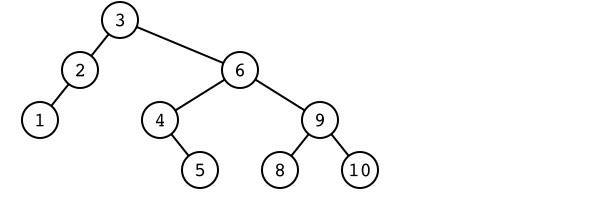
\includegraphics[width=\textwidth]{./figures/bstremoval_example1.png}

\begin{Verbatim}[commandchars=\\\{\}]
\PY{n}{T}\PY{o}{.}\PY{n}{remove}\PY{p}{(}\PY{l+m+mi}{6}\PY{p}{)}
\end{Verbatim}



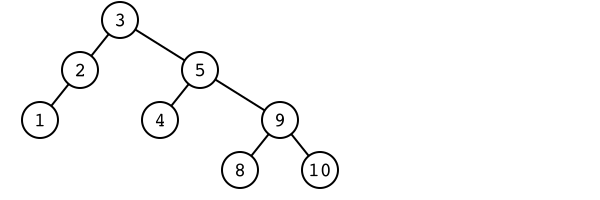
\includegraphics[width=\textwidth]{./figures/bstremoval_example2.png}

\begin{Verbatim}[commandchars=\\\{\}]
\PY{n}{T}\PY{o}{.}\PY{n}{remove}\PY{p}{(}\PY{l+m+mi}{3}\PY{p}{)}
\end{Verbatim}



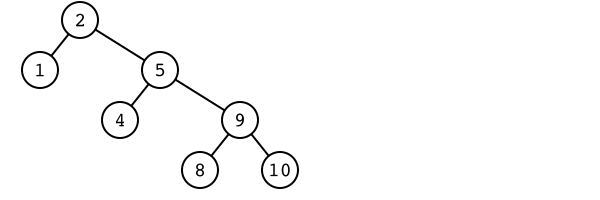
\includegraphics[width=\textwidth]{./figures/bstremoval_example3.png}
